%\documentclass[english]{llncs}
%\usepackage[T1]{fontenc}
\documentclass[10pt, a4paper]{article}
\usepackage{lrec2006}
\usepackage{framed}
\usepackage{graphicx}
%\makeatletter

%%%%%%%%%%%%%%%%%%%%%%%%%%%%%% LyX specific LaTeX commands.
%% Bold symbol macro for standard LaTeX users
\providecommand{\boldsymbol}[1]{\mbox{\boldmath $#1$}}

%% Because html converters don't know tabularnewline
\providecommand{\tabularnewline}{\\}

%\usepackage{babel}
%\makeatother

\title{Efficient Minimum Perfect Hash Language Models}

\name{David Guthrie, Wei Liu}

\address{Department of Computer Science, University of Sheffield\\
		D.Guthrie@dcs.shef.ac.uk, W.Liu@dcs.shef.ac.uk}

\abstract{
The recent availability of large collections of text such as the Google 1T 5-gram corpus \cite{GoogleWeb1T} and the Gigaword corpus of newswire \cite{Graff2003} have made it possible to build language models that incorporate counts of billions of $n$-grams.  This paper proposes a new method of compactly storing language models that allows O(1) random access and uses significantly less space than all known approaches.  We make use of minimal perfect hashing to store fingerprints of $n$-grams in an approach similar to that used by \newcite{talbot1}, but allowing full $n$-gram probabilities to be stored in 63\% of the space that would be required using their approach.  We also show that our approach can easily be combined with block compression, entropy based pruning, and quantization to achieve additional reductions in the size of the language model.
}

\begin{document}
\maketitleabstract

\section{Introduction}
Determining the most probable sequence of words is an integral part of many natural language processing tasks, such as machine translation and speech recognition.  The probabilities of these possible sequences of words are represented using a language model.  Typically language models store $n$-grams of each distinct sequence of words up to length n that occur in a collection of training documents and associate with each of these sequences a frequency count or a probability.  Increasing the size of the training data used has been shown to be a very beneficial way of improving the performance of a language model.  This has lead to the use of larger and larger corpora to create better language models. 

Recent work by \newcite{Brants-2007} showed that machine translation quality continues to significantly improve even when increasing the language model training size above 1 trillion tokens and leading to the conclusion that further gains are still to be had by increasing the size of language models.  Storing these models so that they can be accessed quickly has become problematic due to the space required for these large models.   Language models have commonly been stored in compact trie structures that allow fast searching and enumeration of $n$-grams, yet these structures do not scale well and require space proportional to both the number of $n$-grams and the vocabulary size.

Recent work into random access models \cite{Talbot07smoothedbloom,talbot1,talbot-osborne:2007:ACLMain} has made significant advanced in reducing the amount of space required to store a language model. They make use of the idea that it is not necessary to actually store $n$-grams in the language model as long as when queried with an $n$-gram the model returns the correct count or probability associated with that $n$-gram.  This is achieved through the clever use of Bloom filters \cite{bloom} that trade a very small probability of returning a false positive for the fact that they can represent data very efficiently.  These techniques allow the storage of language models that are no longer dependent on the size of the vocabulary, but only on the number of $n$-grams.  We build upon this work using recent advances in perfect hash functions and making use of the zipf-like distribution of words in language to further reduce the size of storing a language model.  We achieve this reduction in space without increasing the time required to store the model or increasing the time required to query the model for an $n$-grams probability or increasing the false positive rate.  Additionally our model scales better, allowing for the storage of more accurate probabilities or additional counts with no additional space overhead required.  Our method achieves storage of language models using only 2.76 Bytes per $n$-gram with O(N) construction time and O(1) lookup time.  Additionally, in the full paper we show that if block compression techniques are applied we can further reduce the size of the language model by sacrificing a small amount of lookup time.

\section{Related Work}

Many other lossy methods exist for reducing the size of a language model by storing less information. Many of these techniques can be seen as complementary and can be used with any structure (including ours) for further reductions in the size of the language model.  For instance it is possible to reduce then number of $n$-grams that must be stored in the model using entropy pruning techniques \cite{Stolcke98entropy} or clustering \cite{Jelinek90self-organizedlanguage,Goodman00l} and it is also possible to reduce the amount of bits required to store each $n$-grams associated probabilities or counts by sacrificing some precision using quantization \cite{quantization}.  This paper focuses on the data structures that are used to store these $n$-grams and their probabilities whether or not they have first been pruned or quantized.  

Language models have typically been stored using compact trie structures, but more recently methods have been proposed using hash like data structures that allow random access and achieve significant space savings.  In this section we give a brief overview of both approaches, highlighting the advantages and disadvantages of each.

\subsection{Trie based language models}
Most modern language modeling toolkits including SRILM \cite{Stolcke02srilm-}, CMU toolkit \cite{cmu}, and MITLM \cite{paul} currently store their language models using a trie data structure \cite{fredkin}.  This is a compact tree structure where each node stores the unique prefixes of the nodes below it in the tree.  For $n$-gram language models these prefixes are typically 24 or 32 bit integers that represent words (typically all words in the vocabulary are assigned a distinct integer representation).  So every  node in the trie along with its parent nodes represents a distinct $n$-gram.  The probabilities or counts associated with an $n$-gram can be stored in the tree node along with the word.  Very compact representations of these structures have been devised that do not require storing pointers and are used in the CMU toolkit (described in \newcite{quantization}) as well as the MITLM and others \cite{harb,joanis}.  Tries allow the model to be stored in relatively little space and they also permit enumeration over $n$-grams in the model.  For instance it is possible to list all $n$-grams in the model or to query the model for $n$-grams that begin with certain words and iterate through all of the results.  

The main drawback of the trie approach is that it needs to store a representation for every word in the $n$-gram and the probabilities.  Even using 24 bit integers for words in the vocabulary and quantizing probabilities to 8-bit integers, this model requires significantly more space that the random access approach described in the next section.  The size of the trie model can be reduced using block compression as in \newcite{harb}, but this technique can equally be applied to random access models if this increase in the time required to query the model is acceptable.

\subsection{Random Access Language Models}
Random access language models \cite{Talbot07smoothedbloom,talbot1,talbot-osborne:2007:ACLMain} make use of hash functions to map $n$-grams to their associated probabilities or counts.  These structures do not allow enumeration over the $n$-grams in the model, but for many applications this is not a requirement and their space and speed advantages make them extremely attractive.  These methods store language models in relatively little space by not actually storing the $n$-gram key in the structure and allowing a small probability of returning a false positive.  In the case of $n$-grams these models always return the correct probability associated with an $n$-gram if the $n$-gram is in the model, but for $n$-grams that are not in the model there is a small probability that the model will return some random probability instead of correctly reporting that the $n$-gram was not found.  There have been two major approaches used for storing random access language models: Bloom Filters and Bloomier Filters.  We give an overview of these approaches below.

A Bloom filter \cite{bloom} is a data structure used in membership queries.  It can be used to answer simple queries of the form ``Is this key in the Set?''.  This is a weaker structure that a dictionary or  hash table which also can associate a value with a key.  Bloom filters use well below the information theoretic lower bound of space required to actually store the keys and can answer queries in O(1) time.  Bloom filters achieve this feat by allowing a small probability of returning a false positive.  A Bloom filter stores a set $S$ of $n$ elements in a bit array $B$ of size $m$.  Initially $B$ is set to contain all zeros.  To store an item $x$ from $S$ in $B$ we compute $k$ random independent hash functions on $x$ that each return a value in the range 1 to $m$.  These values server as indices to the bit array $B$ and  the bits at those positions are set to 1.  So, $B[h_i(x)]=1 \mbox{ for } i=1 \mbox{ to } k$.  We do this for all elements in $S$ storing to the same bit array.  Elements may hash to the an index in $B$ that hash already been set to 1 and in this case we can think of these elements as ``sharing'' this bit.

To test whether the set S contains a key, say $w$, we run our $k$ hash function on $w$ and check to see if all those locations in $B$ are set to 1.  If $w \in S$ then the bloom filter will always declare that $w$ belongs to $S$, but if $x \notin S$ then the filter can only say with high probability that $w$ is not in $S$.  This error rate depends on the number of $k$ hash functions and the ratio of $m/n$.  For instance with $k=3$ hash functions and a bit array of size $m=20n$, we can expect to get a false positive rate of .0027.

\newcite{Talbot07smoothedbloom} and \newcite{talbot-osborne:2007:ACLMain} made use of bloom filters to store a trigram language model by inserting into the bloom filter a concatenation of an $n$-gram and its associated count.  To insert a trigram that occurred $c$ times they inserted the trigram into the Bloom filter $c$ times, each time appending a count from 1 to $c$.  To retrieve a trigram count form the model, a trigram is first queried by appending a count of 1 and then if the filter returns true the trigram is queried again appending a count of 2.  This process is repeated until the filter returns false.  They limit this process by quantizing all counts to 8-bits so there are a maximum of 256 iterations that must be tried.  The Zipf-like distribution of language means that many of the $n$-grams in the test data will occur a small number of times, so for most lookups the iteration count is small. 

More recently \newcite{talbot1} proposed the use of the Bloomier filter for storing language models.  A Bloomier Filter \cite{bloomier} is a membership testing data structure that allows values associated with the keys to be retrieved from the filter.  Bloomier Filters generalize the Bloom Filters to encode arbitrary functions while maintaining their economical use of storage.  For details on the construction of Bloomier Filters see \newcite{bloomier,talbot1}.  The Bloomier filter is used by \newcite{talbot1} to store for each $n$-gram an associated probability.  Like the Bloom filter, the Bloomier filter has a small probability of returning an incorrect result when queried with an $n$-gram that does not exist in the model, but will always return the correct probability if the $n$-gram is in the model.

The Bloomier Filter can be thought of as a Perfect Hash Function \cite{Botelho1997} and this is a helpful way of understanding how it trades some probability of false positives for efficient storage.  A Perfect Hash Function is a function that maps distinct the $n$ distinct elements of $S$ to distinct integers in the range 1 to $r$ with no collisions.  (A \emph{minimum} perfect hash function, used in the next section, is a function that can do this with $n=r$, see Fig.~\ref{fig:method}.)  We can think of a Bloomier language model as consisting a perfect hash function $ph()$ that maps $n$-grams to integers in the range 1 to $r$ and then storing at that index in an array $A$ a fingerprint and a value.  The fingerprint is generated by a standard independent hash function and the value is the probability or count associated with that $n$-gram.  The amount of bits we keep for the fingerprint determines the false positive rate for $n$-grams not in the model.  Storage of the fingerprint is necessary if we know that the model might be queried for $n$-grams not in the model.  This is because the perfect hash function $ph()$ will likely map unseen trigrams to some index in $A$ and only by comparing the fingerprints can we say with high probability whether that $n$-gram was actually in the model.  \cite{talbot1} give results of using this model for Machine Translation experiments using 8 to 12 bit fingerprints and storing 5 to 8 bit quantized probability values.  Quantization divides the 
probability range into $Q$ discrete values. Each $n$-gram probability is 
therefore`rounded' to one of the $Q$ values, by doing so each probability value 
only requires $\log_2{Q}$ bits to store.


\begin{figure}[htp]
\protect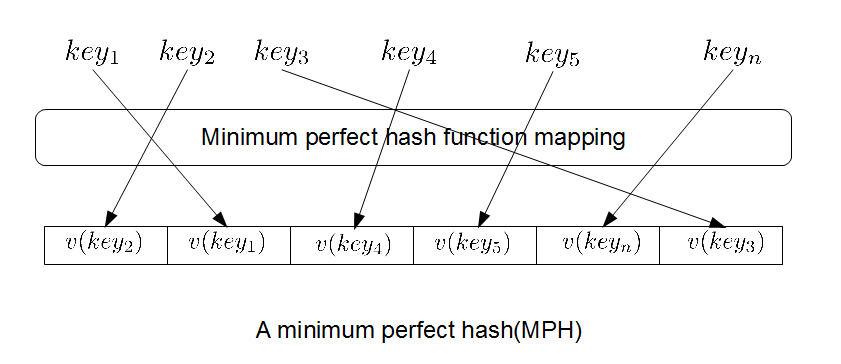
\includegraphics[scale=0.3]{pics/mph}
\caption{A minimum perfect hash function maps keys to integers in the range 1 to $|keys|$}
\label{fig:method}
\end{figure}

\section{Minimum Perfect Hash Ranking Approach}

We propose a data structure called Minimum Perfect Hash Rank (MPHR) that is more compact than that of 
~\newcite{talbot1} while still keeping a constant look up time. Similar to ~\newcite{talbot1} we do not store $n$-grams directly, we map each $n$-gram that 
we want to store using a perfect hash function.  This hash function associates 
each $n$-gram to its $fingerprint$ and value. The function will always return the correct associated value for each stored $n$-gram, but it will also return a mapping for each $n$-gram that is never stored, so it is necessary to store the additional fingerprint to reduce the probability of getting false positives.


 We describe our storage of the values associated with $n$-grams in our model assuming we are storing frequency ``counts'' of $n$-grams, but it applies equally well to storing quantized probabilities.  For the values of the $n$-grams, we store the `rank' of the frequency
count $r(key)$, ($r(key)\in [0..R-1] $) and have a separate array to store the actual counts where the index of the array is the `rank'. This is similar to quantization but allows more accurate information to be stored in less space.  This was motivated by the Zipf-like distribution of $n$-gram frequency counts in corpora.  For example, the number of $n$-grams that occur $1$ time 
is approximately $2$ times more than $n$-grams that occur $2$ times. 
As a result, in a $N$ sized $n$-gram language model, for the distinct number of 
frequency counts are $R$,  we have $R \ll N$.  In our cleaned Google Web1T trigram data, we counted 480 million distinct trigrams yet there are only $330,000$ distinct frequency count.  Because we only store the frequency rank, to keep the precise frequency information we will need $\log_2{R}$ integers. Using quantization of counts or probabilities to $Q$ values, our method will at most require $\log_2{Q}$ bits per $n$-gram and likely less.

We use the CHD minimum perfect hash function described in \cite{CHD-2009} to generate a perfect hash function that only requires $2.07$ bits per $n$-gram.
So for a $N$ sized $n$-gram language model the hash function takes up $2.07*N$ bits.
After this an $N$ sized array is needed to store the $fingerprint$ and values (counts) of each $n$-gram. Let us
further assume that the $N$ sized $n$-gram model has a total $K$ distinct frequencies counts ($K \ll N$),
we will need another $K$ sized array $R[r(key_1)]..R[r(key_n)]$ to store each frequency count (each being a 32bit integer), Figure~\ref{fig:model} shows the overall structure of our model.  
%
\begin{eqnarray}
2.07*N+fingerprint*N+log_2{K}*N+K*32 
\end{eqnarray}
bits to store the entire model.
%
\begin{figure*}[tbp]
\centering
\protect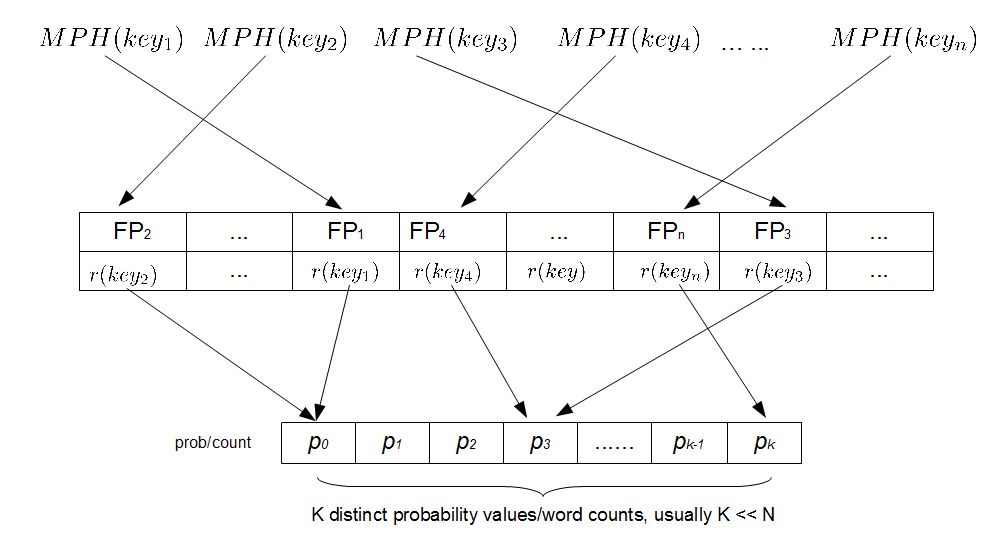
\includegraphics[scale=0.35]{pics/model}
\caption{Storing a very large $n$-gram language model}
\label{fig:model}
\end{figure*}
%
To look up an $n$-gram, we will first find the $fingerprint$ stored in the position given by the perfect hash function, then we check whether the $fingerprint$ of this $n$-gram matched the stored $fingerprint$. If yes then we return its $rank$, and another look-up into array $R[rank]$ and return the stored value, this will be the frequency or probability of the $n$-gram. Clearly both look ups are order $O(1)$.

Table ~\ref{table:usage} and ~\ref{table:comparison} show the bytes per $n$-gram requirement our MPHR model compared to other methods.
%
\begin{table*}[tbp]
\centering
\begin{tabular}{|c|c|c|c|c|}
\hline
 $fingerprint$&prob/count&RPH&MFHR& savings\\
%\hline
\multicolumn{2}{|c|}{bits}&\multicolumn{2}{|c|}{bytes/$n$-gram}&\\
\hline
12 & 8 &  3.08  &  2.76   & 10.28\% \\
12 & 12 &  3.69 &  3.26   & 11.69\% \\
12 & 20 &  4.92  &  4.26   & 13.44 \% \\
12 & 32 &  6.77  &  5.75   & 14.87 \% \\
\hline
16 & 8 &  3.69  &  3.26   & 11.69\% \\
16 & 12 &  4.3 &  3.76   & 12.69\% \\
16 & 20 &  5.54  &  4.76   & 14.02 \% \\
16 & 32 &  7.38  &  6.26   & 15.19 \% \\
\hline
\end{tabular}
\caption{Comparison between \newcite{talbot1} RPH and our proposed MFHR method}
\label{table:usage}
\end{table*}
%
Note that the randomized perfect hash method introduces a 1.23 bits/$n$-gram overhead.
%
\begin{table}[tbp]
\centering
\begin{tabular}{|c|c|}
\hline
Method&Space\\
&bytes/$n$-gram\\
\hline
SRILM Compact&33.6\\
CMU 32b, Quantized&7.2\\
CMU 24b, Quantized&6.2\\
RPF & 5.12\\
MPHR & 2.76\\
\hline
\end{tabular}
\caption{Comparison between different language model storage representations}
\label{table:comparison}
\end{table}
%
The CMU Quantized method uses an 8-bit quantization, in our MPHR method we use 12b-$fingerprint$,
8bit quantization.
%
Although our MPHR require an additional array $R$ of $K$ elements to store the frequencies, 
this array is very small since $K\ll N$ and in a typical large $n$-gram language model its memory
usage is insignificant.


\bibliographystyle{lrec2006}
\bibliography{lrec2010}

\end{document}

